\documentclass{report}
\usepackage{graphicx}
\usepackage[fleqn]{amsmath}
\usepackage[utf8]{inputenc}
\usepackage[fontsize=15pt]{fontsize}
\usepackage{ragged2e}
\usepackage{blindtext}
\usepackage{hyperref}
\usepackage{xcolor}
\usepackage{listings}
\usepackage{url}

\title{\textbf{ME5010 : Logistic Map}}
\usepackage{geometry}
 \geometry{
 a4paper,
 total={170mm,257mm},
 left=20mm,
 top=20mm,
 }
\begin{document}
\author{Shyam Sridhar\\ Nitesh Singh \\ Rudramuni TS \\ Pavan Kumar \\ Aman Gautam }
\maketitle

\section{Introduction}
\raggedright

\begin{center}$x_{n+1} = rx_n(1-x_n)$\end{center}
Logistic Equation is primarily know for modeling population growth of animals and it is part \textbf{Chaos Theory}, which is branch of mathematics that demonstrates how deterministic mathematical system could lead to unpredictability.

Logistic equation is characterized by it's sensitivity to input parameters. Very small changes in $x_0$ and $r$ could lead to drastic changes in predictions, and thus leading to Chaos. Due to this particular nature logistic map was once used to generate array of seemingly unrelated numbers also called pseudo-random number. It could generate unpredictability from deterministic machine. Beside that it is also used in cryptography for encryption of data where encrypted data would be very sensitive to the key i.e small variation in key would not decrypt/decode the encrypted data allowing only one and one unique key to decrypt the data.

In this project our aim is to explore behaviour of logistic map. It's sensitivity to initial parameters, period doubling, unpredictability and device a pseudo-random number generator (PRNG). We will use same PRNG to encrypt an image.

\section{Uniformity in Randomness}
\raggedright

Reason why I use \textbf{pseudo}-random numbers because for exactly same starting conditions or initial values we will have same array of numbers that are deterministic. As a matter of fact even pre-built random number generator in python also gives same array of numbers if we query random numbers with a particular seed or initial parameter.

The idea behind generating pseudo-random numbers from such system is their sensitivity  to initial conditions itself. Even change in orders of $10^{-6}$ would generate an entirely different array of numbers. Determining the seed or initial condition is not straight-forward given a state of certain point in future. Moreover, explaining systems that are hypersensitive to initial parameters is forte of Chaos Theory

\begin{quote}
When a butter fly flutters it's wings in one part of the world, it can eventually cause a hurricane in another.  (Edward Norton Lorenz)
\end{quote}


\newpage
\section{Logistic Equation}
\raggedright
The following equation also called logistic equation is used to model population growth.
\begin{equation}
x_{n+1} = rx_n(1-x_n) \nonumber
\end{equation}
where:

$x_n$ = population in $n$th generation,

$r$ = growth rate

\begin{figure}[!h]
    \centering
    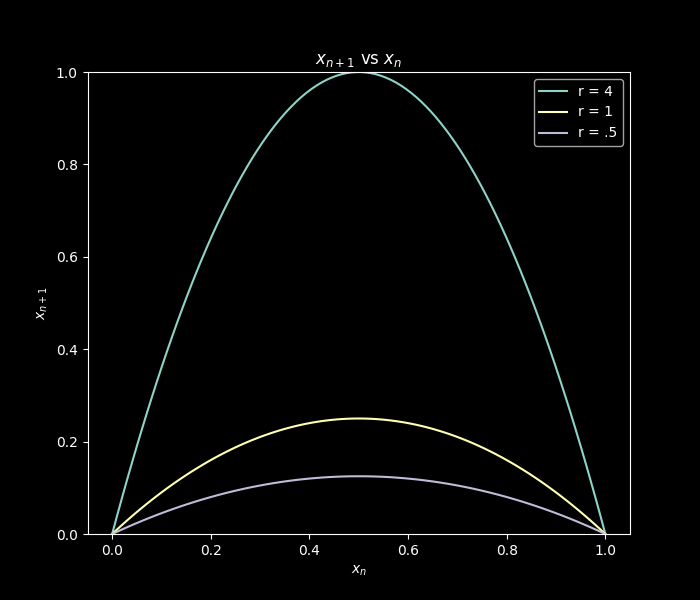
\includegraphics[scale=.5]{images/xnvsnp1.png}
    \caption{$x_{n+1}$ vs $x_n$ (Such functions are also called single humped functions)}
    \label{fig:my_label}
\end{figure}

For $r \in [0, 4]$ the function $x_{n+1}$ maps the closed interval [0, 1] into itself. We shall
restrict our attention to these values of r. Also we'll see r is the main factor contributing to unpredictability of equation.

As observed from the graph below $x_{n}$ is not exactly predictable for every r.

\begin{figure}[!h]
    \centering
    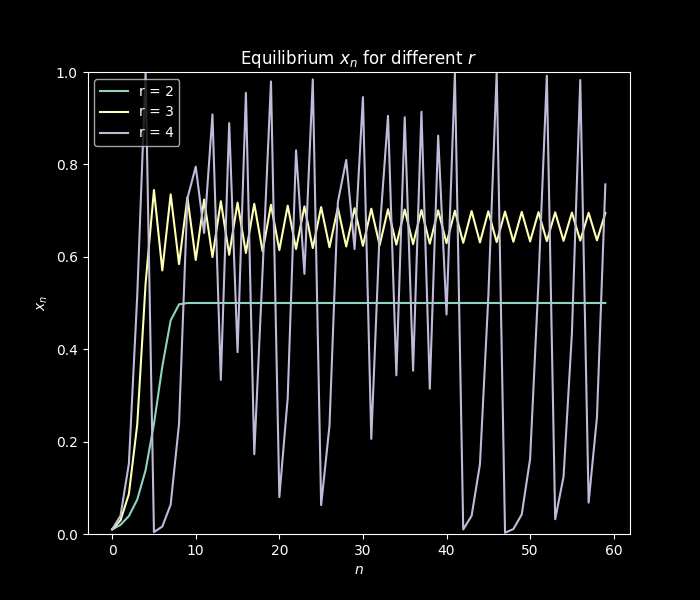
\includegraphics[scale=.4]{images/eqfordifr.png}
    \caption{$x_n$ at equilibrium for different r's}
    \label{fig:my_label2}
\end{figure}

On varying r and plotting equilibrium $x_{n}$ we get the following observations.

\begin{itemize}
  \item $r < 3$ One Equilibrium position of x is seen.
  \item $r > 3$ Two Equilibrium position of x is seen.
  \item As r is increased further we have multiple equilibrium positions
\end{itemize}
\newpage
\subsection{Fixed Points}

\raggedright

Equation can be said to be converging when. $x_{n+1} \to x_n$

Thus, we can write
\begin{equation}
    x = rx(1-x) \nonumber
\end{equation}

From above equation we get the following solutions or equilibrium points.\\

$x = 0$ and $x = 1 - \frac{1}{r}$
\begin{itemize}
  \item For $r \in [0,1)$ $x = 0$ acts as attractor (solution converges to this point)
  \item For $r = 1$, $x = 0$ acts as repellor (x seems to diverge from x = 0 line)
  \item And $x = 1 - \frac{1}{r}$ is an attractor for $r \in (1,3)$ and a repeller for $r > 3$.
\end{itemize}


This can be obtained from the slope of $f_r = rx(1-x)$ at x, \newline
that is equal to $r(1-2x)$. For points 0 and $1-\frac{1}{r}$.
\begin{align}
    &f'_r(0) = r  \nonumber \\
    &f'_r(1-\frac{1}{r}) = 2-r \nonumber
\end{align}

Absolute value of Slope less than 1 implies $x_n$ will be attracted to the solution and vica-versa. Observe there is no single point attractors for $r>3$ thus explaining why there is no single solution in that case.

In fact, as r continues to increase after 3, $x_n$ converges to a permanent oscillation between two values depending on r. Increasing r further it starts oscillating between 4 values and so-on. This brings us to our next topic of \textbf{period-doubling} observed in logistic equation. This also connects logistic equation with mathematical fractals.
\newpage
\subsection{Period Doubling}
\raggedright
In this section we will see why actually solution starts oscillating between multiple points and doubles with r.
\begin{align}
    &f_r = rx(1-x) \nonumber  \\
    &fof_r = rf_r(1-f_r) \nonumber
\end{align}

For convergence, we will try to find solution of the following equation.
\begin{align}
   & fof_r = x  \nonumber\\
   & x(rx-r+1)(r^2x^2 - (r^2+r)x+(1+r)) = 0 \nonumber
\end{align}

Solving and simplifying this equation we get two other solutions which are roots of the following equation,
\begin{align}
& r^2x^2 - (r^2+r)x+(1+r) = 0 \nonumber \\
& x^2 - (1+\frac{1}{r})x + \frac{1}{r^2} + \frac{1}{r} = 0
\end{align}


If $q_1$ and $q_2$ are solutions of the above equation then they can be real if
\begin{equation}
    (\frac{r+1}{r}) \geq \frac{4(1+r)}{r^2} \nonumber
\end{equation}
This on simplification leading to \newline

$r \geq 3$. This makes sense because cycle of period 2 exist after r = 3 \newline
Again to find where equilibrium is attracted to we will find slope of $f'_r(q_1)f'_r(q_2)$ and find values of r for which it's slope $\in [-1,1]$ where $f'_r = r(1-2x)$
\begin{align}
f'_r(q_1)f'_r(q_2) &= r^2(1 - 2q_1)(1 - 2q_2) \nonumber \\
 &= r^2(1 - 2(q_1+q_2) + 4q_1q_2) \nonumber
\end{align}

Using (1) in this equation
\begin{equation}
f'_r(q_1)f'_r(q_2) = -r^2 + 2r + 4
\end{equation}
We will use same logic that absolute value of slope should be less than 1, for a point to act as an attractor. (That is solution will converge to this point). Here two points ($q_1$,$q_2$) as attractor means solution will converge to two points and hence period doubling.
\newpage

Equation (2) is 1 when $r = 3$, and for $r > 3$  it decreases and reaches value of -1 when $r = 1 + \sqrt[]{6} = 3.449..$
\newline

Thus this shows that solution will oscillate between two points $q_1$ and $q_2$ for values of $r \in (3,3.449..)$

Like this at certain r's we will get period doubling first three are,
\begin{align}
    r_0 &= 1 \nonumber \\
    r_1 &= 3 \nonumber \\
    r_2 &= 1 + \sqrt[]{6} \nonumber \\
    r_3 &= 3.544... \nonumber
\end{align}
This is also called cascade of period doubling, Note  $r_3$ is not evaluated in above calculation I took it from graph I made

Let us define a term which looks like
\begin{equation}
    \delta_k = \frac{r_k - r_{k-1}}{r_{k+1} - r_k}
\end{equation}

For $k = 1$, $\delta_1 \approx 4.44949$ \newline

Graphically we will see this value approaches to \textbf{4.669202...} . This is an universal constant like $\pi$ know as \textbf{feigenbaun's ratio}. It appears in many chaotic system like dripping faucet, firing of neurons in brain, fluid behaviour and is exactly the same.
It is also observed at $r = 3.829$ the equilibrium oscillates in period of 3 because $fofof_r = x$ have three roots. \newline

\begin{figure}[!h]
    \centering
    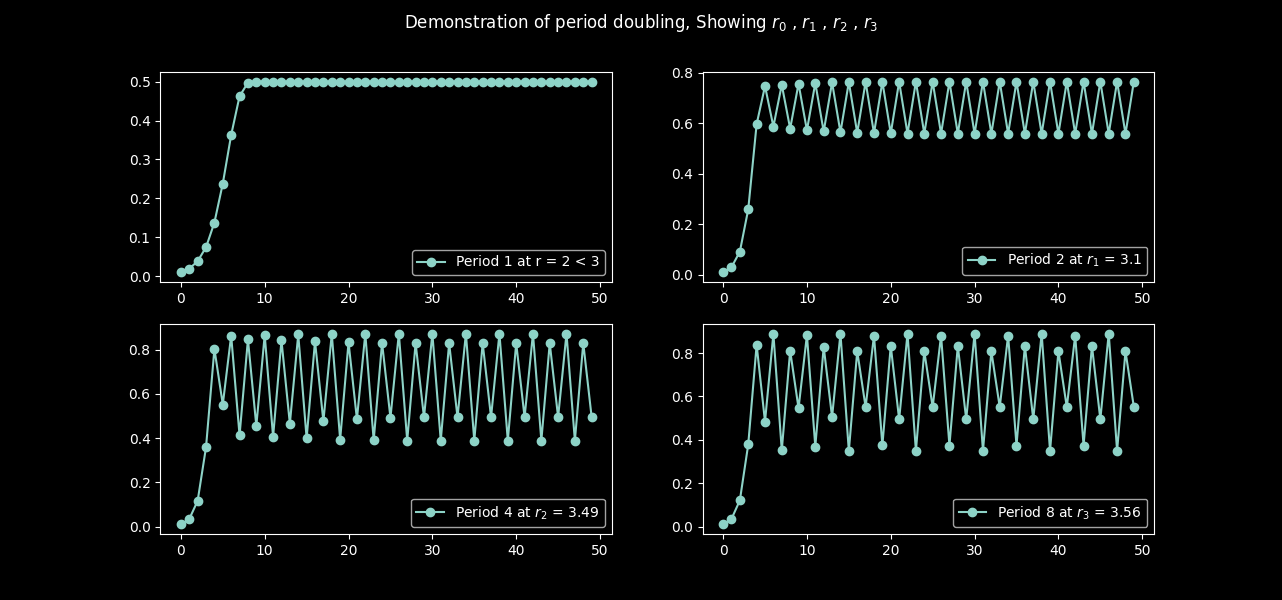
\includegraphics[scale=.45]{images/period2ing.png}
    \caption{Demonstrating period doubling with progression of r}
    \label{fig:my_label3}
\end{figure}

\subsection{Bifurcation Map}
\raggedright
A Bifurcation Diagram is a visual summary of the succession of period-doubling produced as r increases\footnote[1]{https://www.vanderbilt.edu/AnS/psychology/cogsci/chaos/workshop/BD.html}.

In our logistic equation \textbf{r} is the bifurcation parameter and it's show on horizontal axis. The bifurcation diagram shows the forking of the periods of stable orbits from 1 to 2 to 4 to 8 etc. Each of these bifurcation points is a period-doubling bifurcation. The ratio of the lengths of successive intervals between values of r for which bifurcation occurs converges to the first Feigenbaum constant.\footnote[2]{https://en.wikipedia.org/wiki/Bifurcation\_diagram}

\begin{figure}[!h]
    \centering
    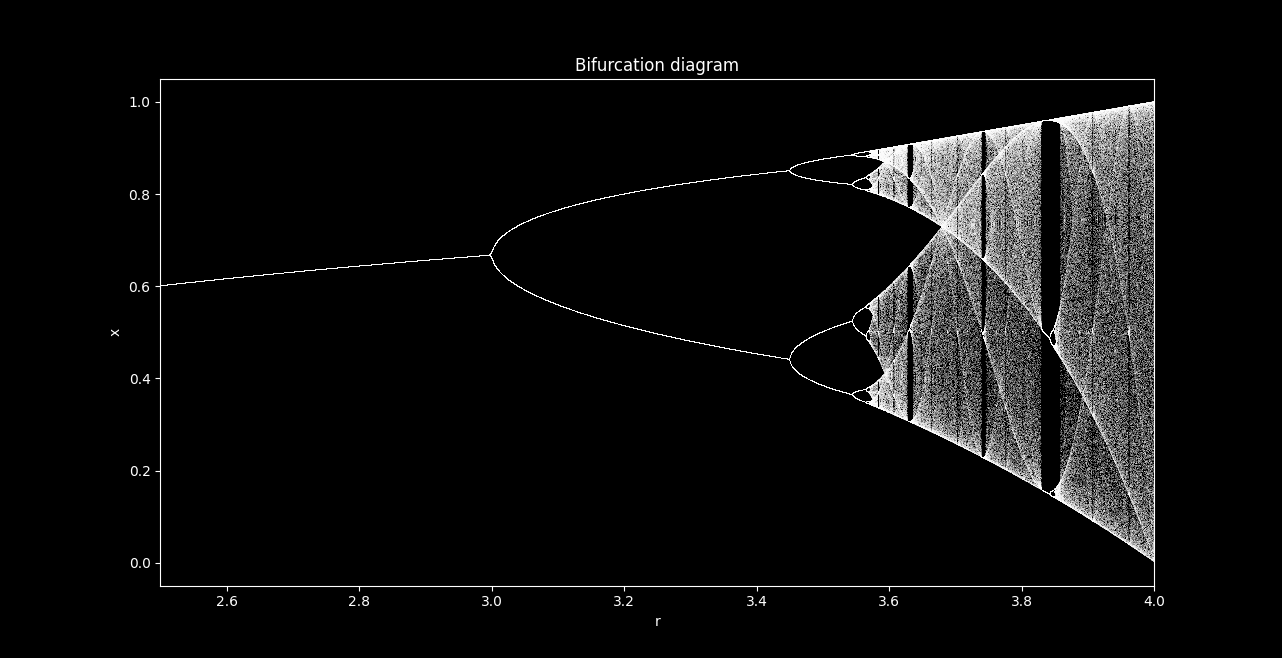
\includegraphics[scale=.45]{images/BifurcationDiag.png}
    \caption{Bifurcation Diagram for $r \in [2.5,4]$}
    \label{fig:my_label4}
\end{figure}

A very high resolution bifurcation map could be generated by running this python code \href{https://github.com/notcamelcase01/ME5010Project/blob/master/high\_res\_bfmap.py}{\textcolor{blue}{Github link}}. The code will plot ten million points and could be zoomed 16x before it becomes sparse.\footnote[3]{Word of caution it's slow for obvious reasons}

The bifurcation map clearly shows occurrence of fractals. Zooming into a part of geometry produces same geometry.

From this Diagram we could find,
\begin{align}
    r_2 &= 3 \nonumber \\
    r_3 &= 3.54409.. \nonumber \\
    r_4 &= 3.56440.. \nonumber \\
    r_5 &= 3.56875.. \nonumber \\
    r_6 &= 3.56969.. \nonumber
\end{align}
\newpage

\begin{figure}[!h]
    \centering
    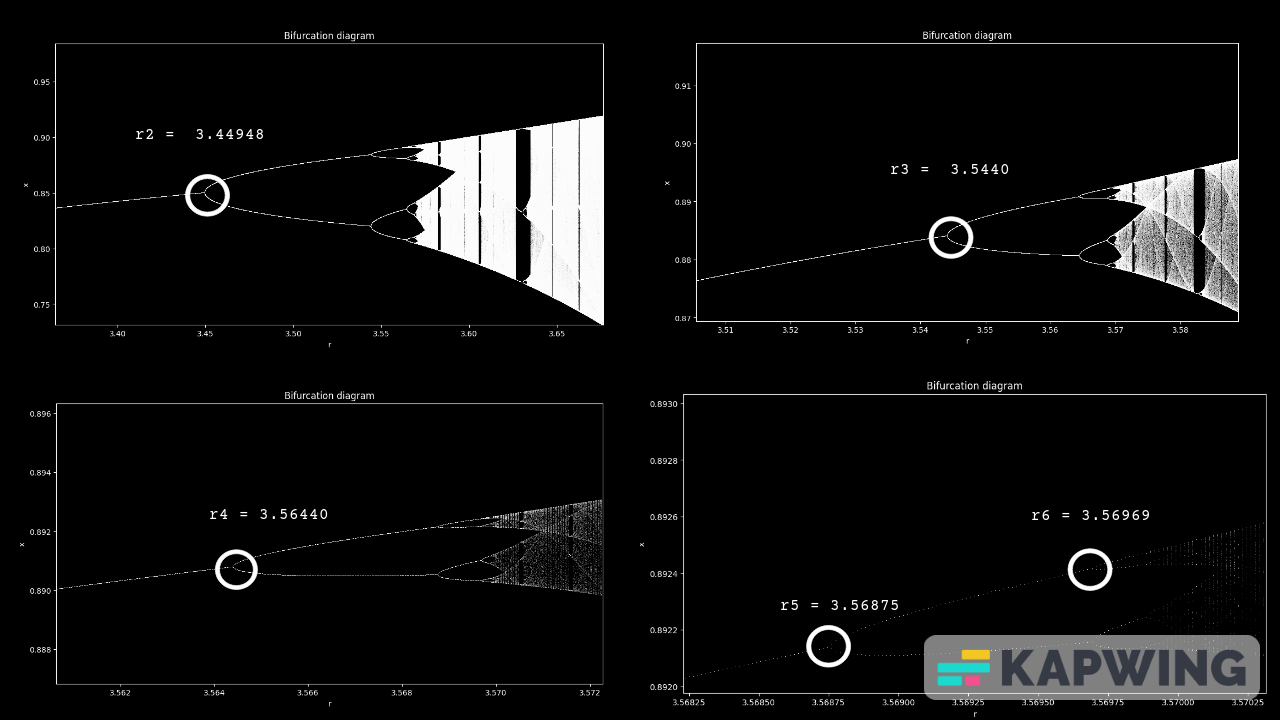
\includegraphics[scale=.35]{images/bfcol.png}
    \caption{Bifurcation Diagram zoom.Top left zoom x2, Top right zoom x4, Bottom left zoom x8, bottom right zoom x16}
    \label{fig:my_label5}
\end{figure}

So what happens if we keep increasing the period, Period at any r can be given by $2^n$, for $r_3$ period is 8.

What about $r_{20}$ ? Graphically it becomes impossible to do this on my computer. Just to give you an idea currently I could zoom to x32 and perhaps I can do it to x64(which would need me to plot 1 billion points) however $r_{20}$ requires x1048576 zoom-able graph so I can read data points.
\newline

Even doing it analytically is tedious like, it's exactly how I did it for $r_2$ for $r_n$ we would have to evaluate $fofofof..ntimesf_r = x$ then obtain its roots in form of r and substitute in $|f'_r(q_1)f'_r(q_2)...f'_r(q_n)| < 1$ then check for what r this polynomial absolute values is more than one.\footnote[1]{I am still working on to find a simpler analytical way but I have failed to find anything for now.}
\newline

Although it is intuitive and seen from data points that $r_n$ is converging to a certain value. \newline

$r_\infty \to 3.5699456....$\footnote[2]{https://documents.uow.edu.au/~mnelson/teaching.dir/discrete.dir/part4.pdf}
\newline

After $r_\infty$ there is no period doubling although it have some regions where period becomes 3 ($r \approx 3.843$). When r reaches 4 the map becomes completely  chaotic a-periodic.
\newpage

\begin{figure}[!h]
    \centering
    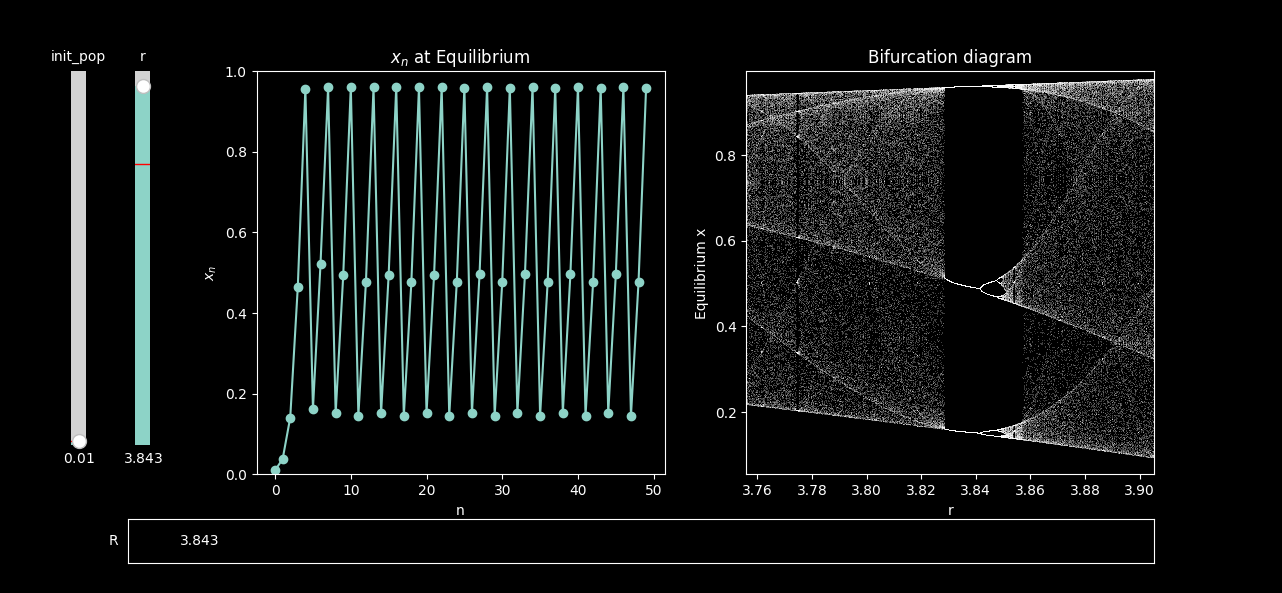
\includegraphics[scale=.45]{images/period3ing.png}
    \caption{Period of 3 at r ~ 3.843}
    \label{fig:my_label6}
\end{figure}

\begin{figure}[!h]
    \centering
    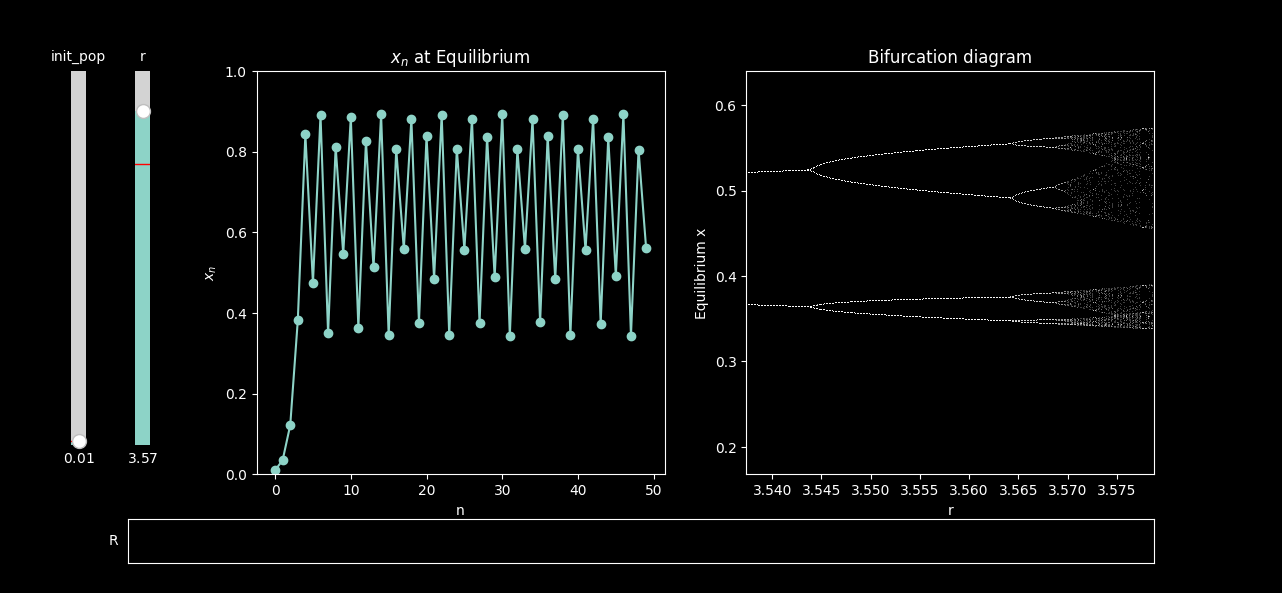
\includegraphics[scale=.45]{images/rinfi.png}
    \caption{State of map around $r_{\infty}$ (Zoomed in)}
    \label{fig:my_label7}
\end{figure}

A summary of what information we know till now,

\begin{itemize}
  \item $r < 1$, solution approaches to 0 quickly.
  \item $r \in [1,3]$ Solution converges to $1-\frac{1}{r}$
  \item $r\in (3,r_{\infty})$ period doubling is observed.
  \item $r\in (r_{\infty},4)$ a-periodicity and chaotic with windows  of 3 period  cycles is observed.
  \item $r=4$ map goes chaotic
\end{itemize}
For pseudo random number generation we are interested in $r \in (r_{\infty},4]$
\newpage

\section{Pseudo-Random Number Generator}

As seen before our logistic map becomes chaotic at r $\in (3.5699,4]$. We will exploit this property of logistic map to generate pseudo-random numbers and do some statistical test on them.

Idea is very simple,
\begin{equation}
    x_{n+1} = rx_n(1-x_n) \nonumber
\end{equation}
This equation will give us series of numbers. Again I will repeat the numbers generated are not truly random they are still generated from deterministic algorithm and thus they are deterministic.
\subsection{Why Pseudo ?}
True random numbers are completely \textbf{irreproducible} while pseudo-random numbers are reproducible, Given the same initial parameters(seed) the algorithm outputs same sets of numbers. The idea is these pseudo-random numbers statistically shows the properties of random numbers and thus could be used in calculations.
\newline

These initial parameters which I talked above are often referred to as seeds. For logistic map we will use initial $x_0$ as seed. So for same seed we will get output of same  numbers which will look like random numbers. Infact, even python function giving "random" numbers uses similar algorithm , so even they would give repeating pattern for same seed.

\begin{lstlisting}
# importing random module
import random

#set seed to 3
random.seed(3)
#generate random number between 0 and 1
print(random.uniform(0,1))
#reset seed to 3
random.seed(3)
#generate random number between 0 and 1
print(random.uniform(0,1))
\end{lstlisting}

Which gives output as $0.23796462709189137$ in both cases. You see for same seed python generates same random number.
\newpage

\subsection{Methodology}
Logistic equation does gives us numbers although they are not uniform within an given interval. To overcome that consider the following map\footnote[1]{https://arxiv.org/pdf/cond-mat/9310004.pdf}
\begin{align}
    &y_n = \frac{\cos^{-1}(1-2x_n)}{\pi}  \\
    &x_{n+1} = 4x_n(1-x_n) \nonumber
\end{align}
$y_n$ will uniformly distribute all the numbers we generate by logistic equation. we will use $x_0$ as our seed parameter.

But before we go an code our PRNG we should remember that logistic map collapses if any $x_0$ becomes 0 or 1 or it attains periodicity.
\begin{align}
    &x_{n+1} = 4x_n(1-x_n) \nonumber \\
    &4x_0(1-x_0) = 0 \nonumber \\
    &4x_0(1-x_0) = 1 \nonumber \\
    &4x(1-x) = x \nonumber
\end{align}
From above equations we get that logistic map will fail to generate pseudo-random numbers if $x$ gets to any of these rational values, $[0 , 0.25 , 0.5 , 0.75 , 1 ]$. Observe that at 0,0.5 and 1 logistic map collapses(r = 4) and for .75 and .25 it attains value of .75

\begin{figure}[!h]
    \centering
    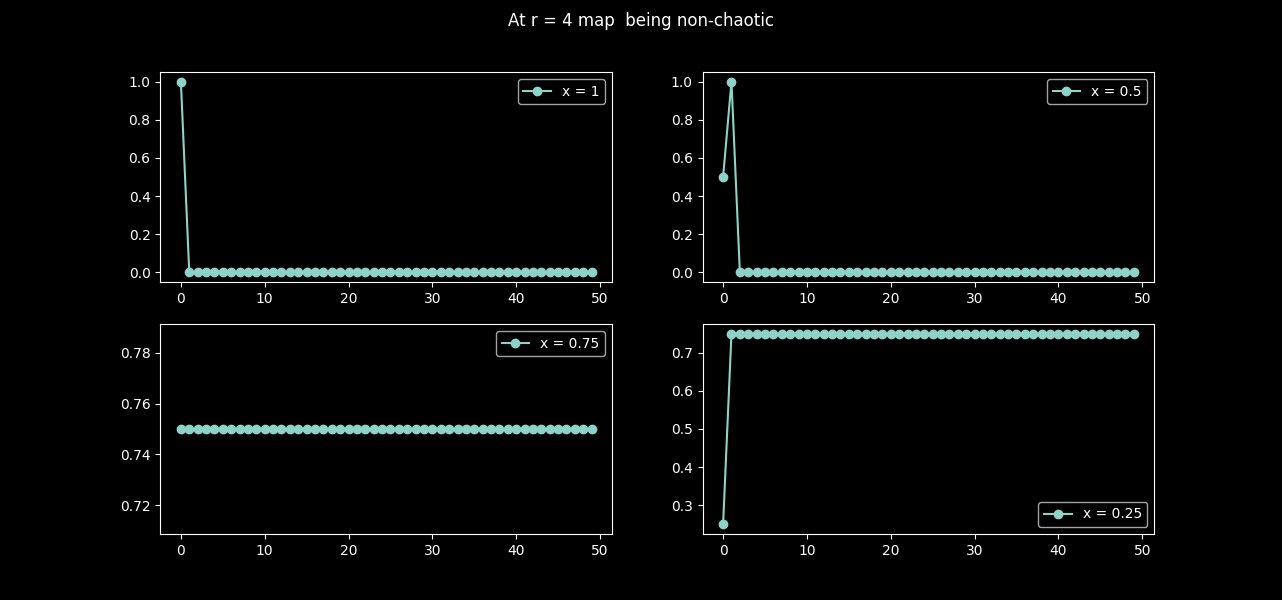
\includegraphics[scale=.45]{images/bummer.png}
    \caption{Non-chaotic starting points at r=4}
    \label{fig:my_label8}
\end{figure}

Thus we will avoid these x to be declared as starting points and our y map (Eq (4)) will ensure all numbers are uniformly distributed.
\newpage
\subsection{Testing Pseudo-random numbers}
After generating random numbers we will compare them with python's random modules random numbers.

The following scatter plot is made using 1000 (x,y) points generated by python's random module on left and logistic map on right.

\begin{figure}[!h]
    \centering
    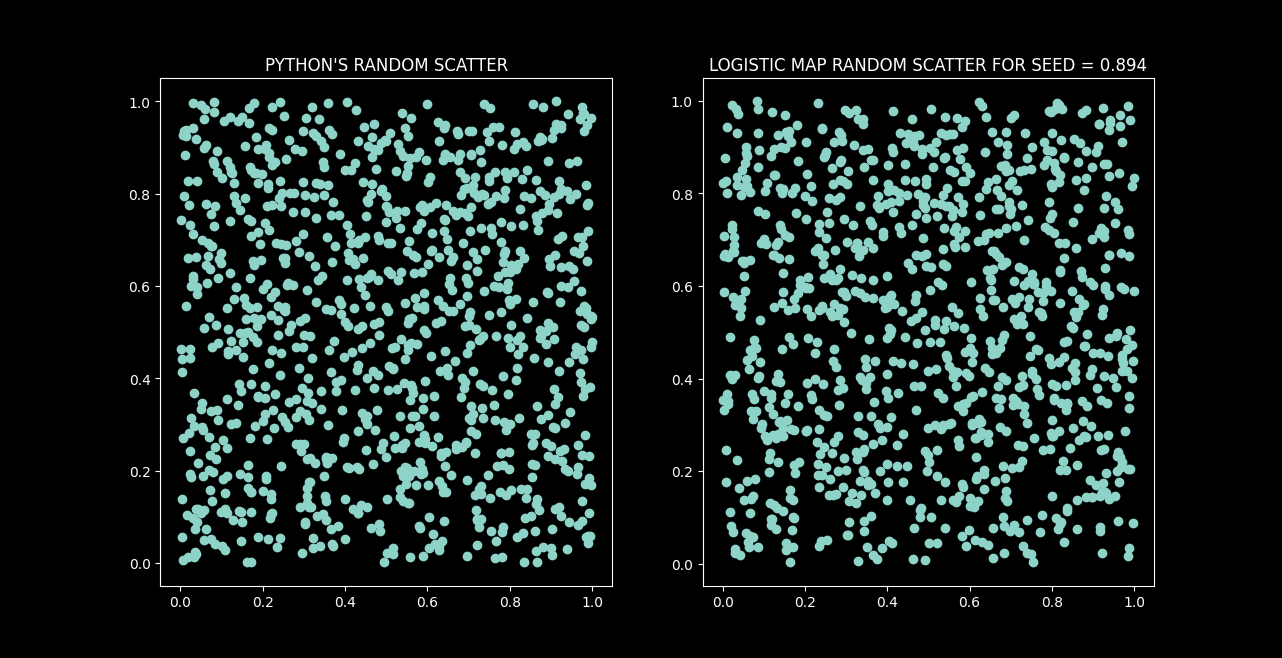
\includegraphics[scale=.45]{images/prngscat.png}
    \caption{Comparing scatter plot for python's and Logistic PRNG}
    \label{fig:my_label9}
\end{figure}

Plotting histogram for logistic random array and python's numpy module random array of 10000 points.

\begin{figure}[!h]
    \centering
    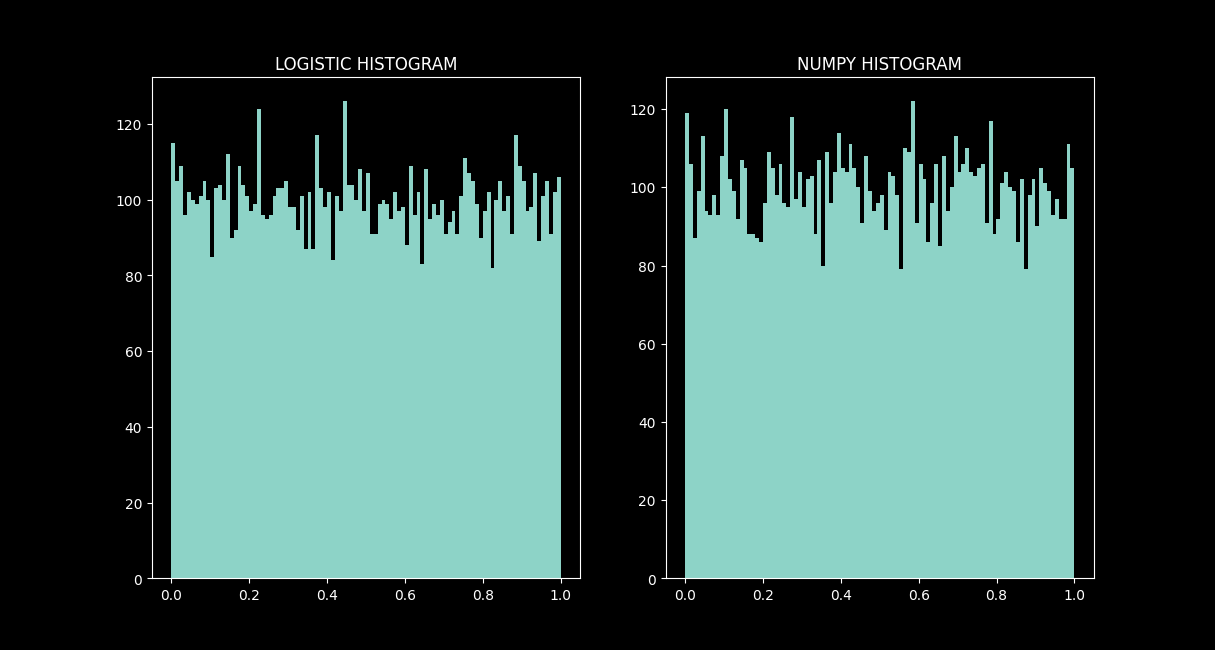
\includegraphics[scale=.45]{images/rndHist.png}
    \caption{Comparing histogram for python's and Logistic PRNG}
    \label{fig:my_label10}
\end{figure}
\newpage

\subsection{Sierpiński triangle}
The Sierpiński triangle (sometimes spelled Sierpinski), also called the Sierpiński gasket or Sierpiński sieve, is a fractal attractive fixed set with the overall shape of an equilateral triangle, subdivided recursively into smaller equilateral triangles.\footnote[1]{Defination from wiki}
\newline
This generated by starting from any of the point inside triangle and then choosing one of the three vertex at \textbf{random} then move towards that vertex by half of the distance between the current point and vertex.Repeat it many times.
Pesudo-random numbers generated from logistic map at r=4 generate this fractal too.(not uniformed)

\begin{figure}[!h]
    \centering
    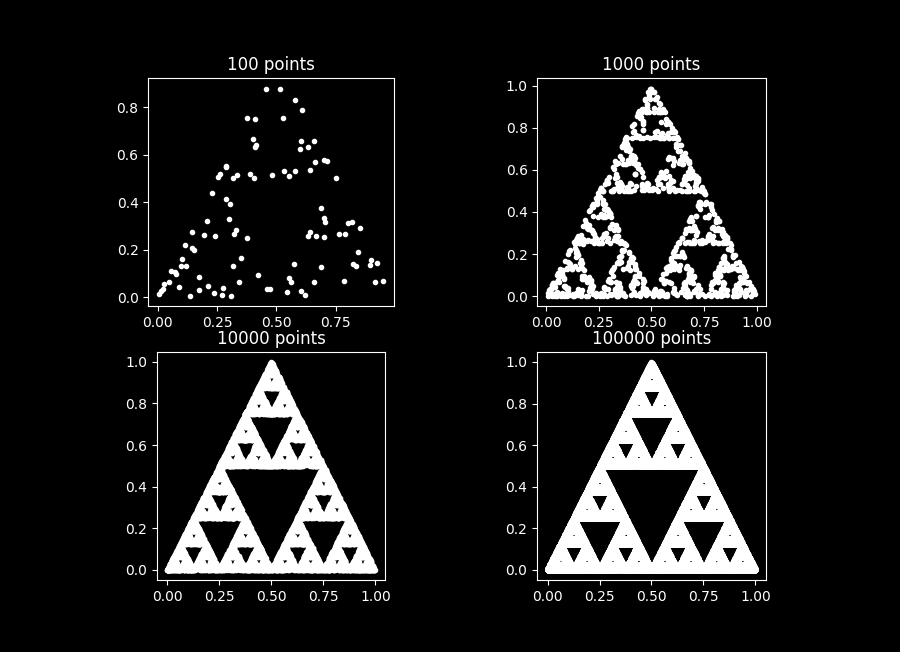
\includegraphics[scale=.4]{images/ilmtri.png}
    \caption{Sierpinski Triangle for different points.(Logistic map)}
    \label{fig:my_label11}
\end{figure}

\begin{figure}[!h]
    \centering
    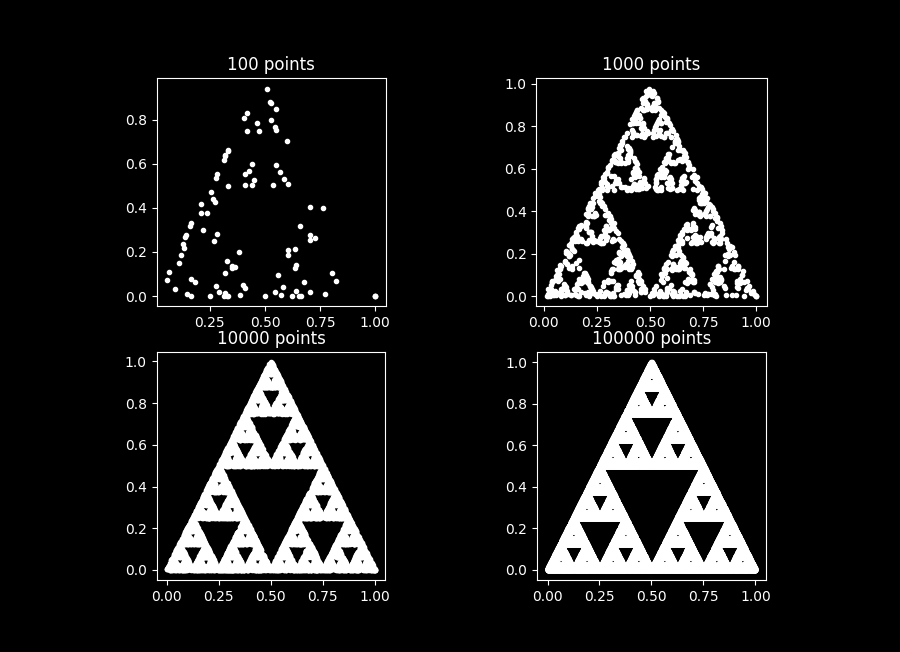
\includegraphics[scale=.4]{images/numpytri.png}
    \caption{For comparision Sierpinski Triangle for different points.(used Numpy random)}
    \label{fig:my_label12}
\end{figure}
\newpage
\section{Image Encryption}

We will try to make image encryption-algorithm using logistic map. The encrypted image could be decrypted by a key, however since logistic map is sensitive to initial parameters we will try to decrypt image using wrong key and see what happens.

\subsection{Methodology}

We took monochrome image where each pixel is 0-256 and generated a random array of integers between 0-256. We will use XOR operation between image pixel and random number to encrypt.

Due to how XOR operator works we can get back original pixel by XORing decrypted image by Key. Key is array of random numbers generated by our PRNG.

\subsection{Results}

\begin{figure}[!h]
    \centering
    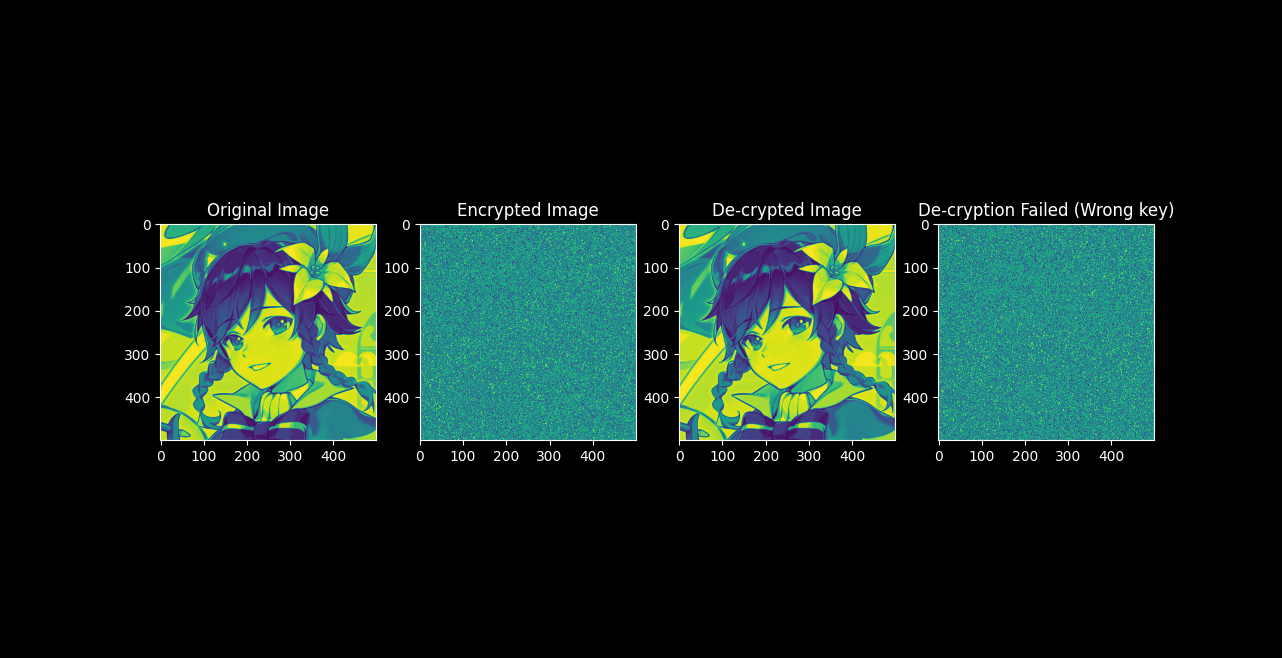
\includegraphics[scale=.4]{images/imageed.png}
    \caption{We differed seed by just $10^{-6}$ and image decryption failed}
    \label{fig:my_labelVenti}
\end{figure}

This not only demonstrate how chaotic maps like logistic equation can be used for data encryption but also shows how sensitive these maps are to initial values.
\begin{quote}
Exact Present can determine exact future but approximate present cannot determine approximate future.  (Fundamentals of Chaos Theory)
\end{quote}

Chaotic maps are used for high-security data encryption in many sensitive areas like banks, showing passwords in database etc


\newpage
\section{Summary}
Logistic map demonstrated how non-linear dynamical equation could lead to unpredictable outcomes. Being highly sensitive to  initial parameters and chaotic in certain regimes it is used for generating pseudo-random numbers. We did generated PRNGs
\newline
PRNG also constructed Sierpinski triangle which is a mathematical fractal. It is one of the Chaos Game.

Altough our logistic based PRNG is not the best, Take this for example. Generation of Barnsley Fern.\footnote[1]{https://en.wikipedia.org/wiki/Barnsley\_fern}
\begin{figure}[!h]
    \centering
    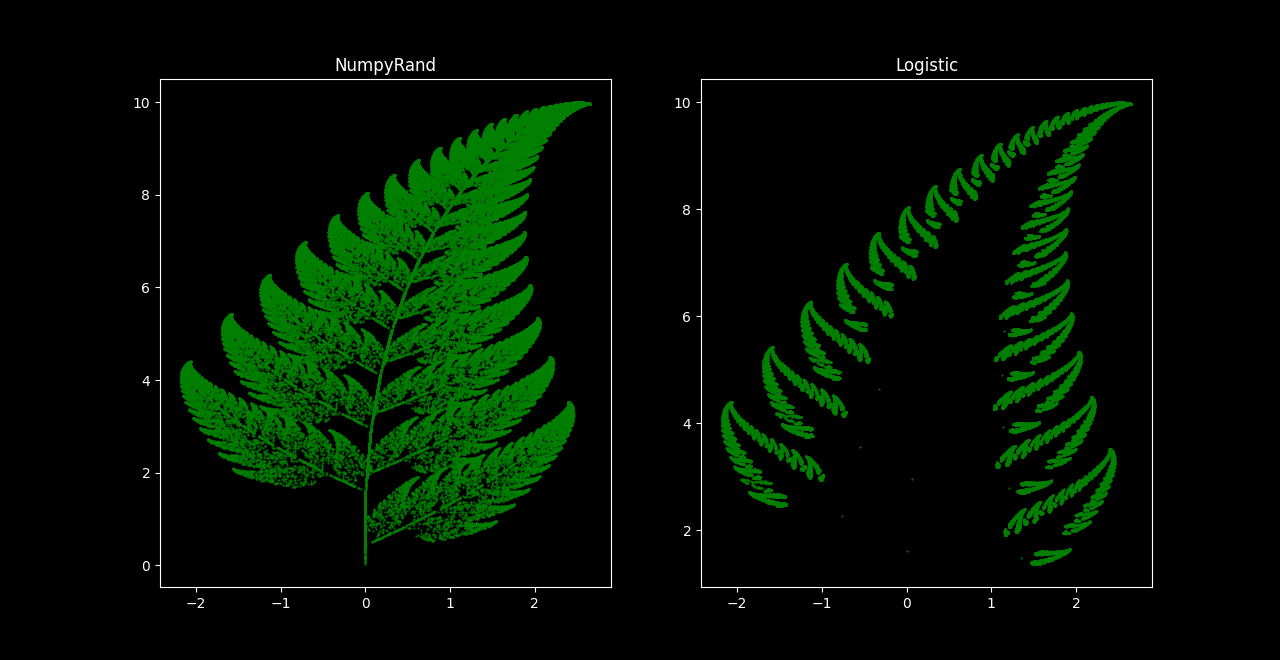
\includegraphics[scale=.3]{images/badfern.png}
    \caption{As you can see PRNG logistic failed to draw fern}
    \label{fig:my_label13}
\end{figure}

But I adjusted the pseudo number generation and used r as seed itself to get this.

\begin{figure}[!h]
    \centering
    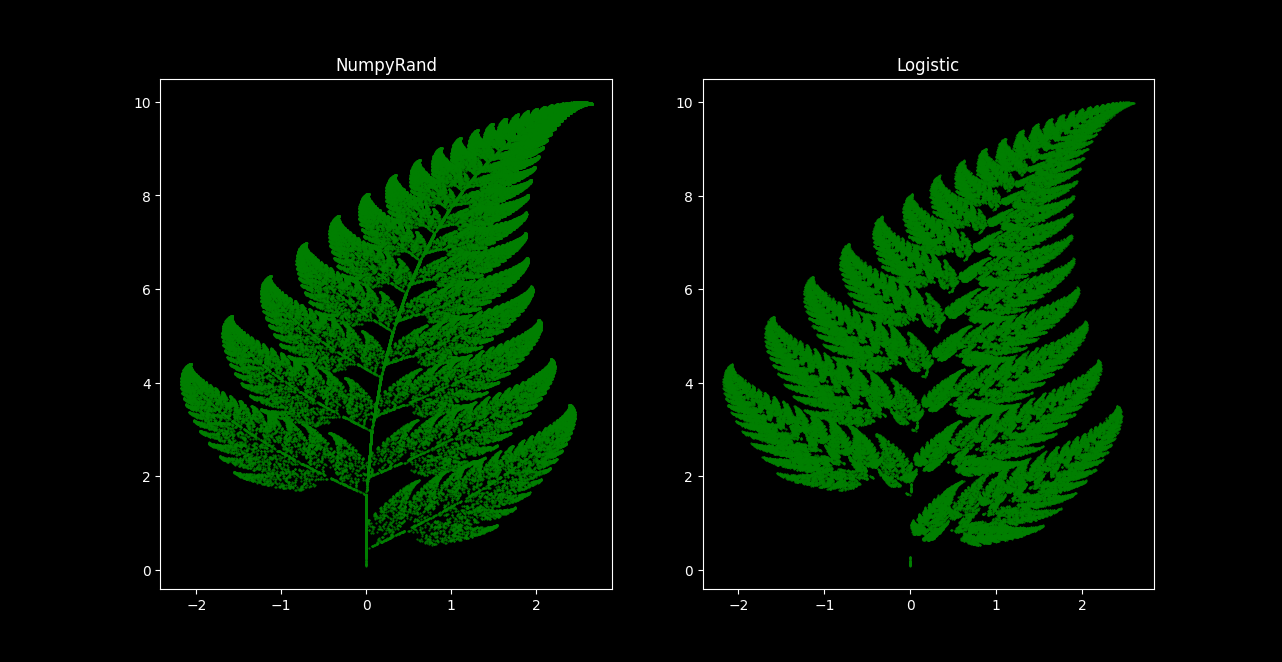
\includegraphics[scale=.3]{images/goodfern.png}
    \caption{Improved PRNG}
    \label{fig:my_label14}
\end{figure}
Not just fern many other natural geometries could be generated by chaos game, like mountains, snow-flake, trees, clouds ,blood vessles , ionization of air (sparking) and list continues. Interesting !!
Nature is chaotic yet so disciplined.
\newpage
\begin{thebibliography}{1}
	\bibitem{r1}
	    S. C. Phatak and  S. Suresh Rao,
		``Logistic Map: A Possible Random Number
Generator;
		1993
	\bibitem{r2}
		Queen Marry University of London,
		\url{https://webspace.maths.qmul.ac.uk/s.r.bullett/cf_chapter3.pdf};
	\bibitem{r3}
		Veritasium youtube video,
		\url{https://www.youtube.com/watch?v=ovJcsL7vyrk&ab_channel=Veritasium};

		\bibitem{r4}
	    Code is written in \textbf{PYTHON}, Link to my Github Repository.  \url{https://github.com/notcamelcase01/ME5010Project}
\end{thebibliography}

\end{document}
